\documentclass[aspectratio=169]{beamer}
\beamertemplatenavigationsymbolsempty
%\setbeameroption{show only notes}
%\setbeameroption{show notes on second screen}

\usepackage{pdfpages}
\usepackage{graphicx}
\graphicspath{{figures}{figures/graphics}}


\usepackage{tikz}
\usepackage{tikzscale}
\usetikzlibrary{shapes, arrows.meta, positioning, calc, intersections}
\tikzstyle{block} = [rectangle, draw, rounded corners]



\usepackage[export]{adjustbox}

\usepackage{caption}
\captionsetup[figure]{labelformat=empty, font=scriptsize, labelfont=scriptsize}

\usepackage{subcaption}
\usepackage{multicol}

\usepackage[numbers, sort&compress]{natbib}
\bibliographystyle{unsrtabbrv}

% beamer style
\setbeamertemplate{blocks}[rounded][shadow]
\setbeamercolor{block body}{bg=structure!10}
\setbeamercolor{block title}{bg=structure!20}

\setbeamercolor{block body example}{bg=green!10}
\setbeamercolor{block title example}{bg=green!20}

\setbeamercolor{block body alerted}{bg=red!10}
\setbeamercolor{block title alerted}{bg=red!20, fg=black}



% just have frame number in footline
\setbeamertemplate{footline}[frame number]

\def\swidth{2cm}
\usetheme[width=\swidth]{Hannover}
%\usecolortheme{}

%%%%% ADD  NOPHOTO Icon

%
\makeatletter
\addtobeamertemplate{sidebar left}{}{%
	\begin{minipage}{\swidth}
		\centering
%		\includegraphics[width=0.3\textwidth]{../../../pres-images/no-photo}
		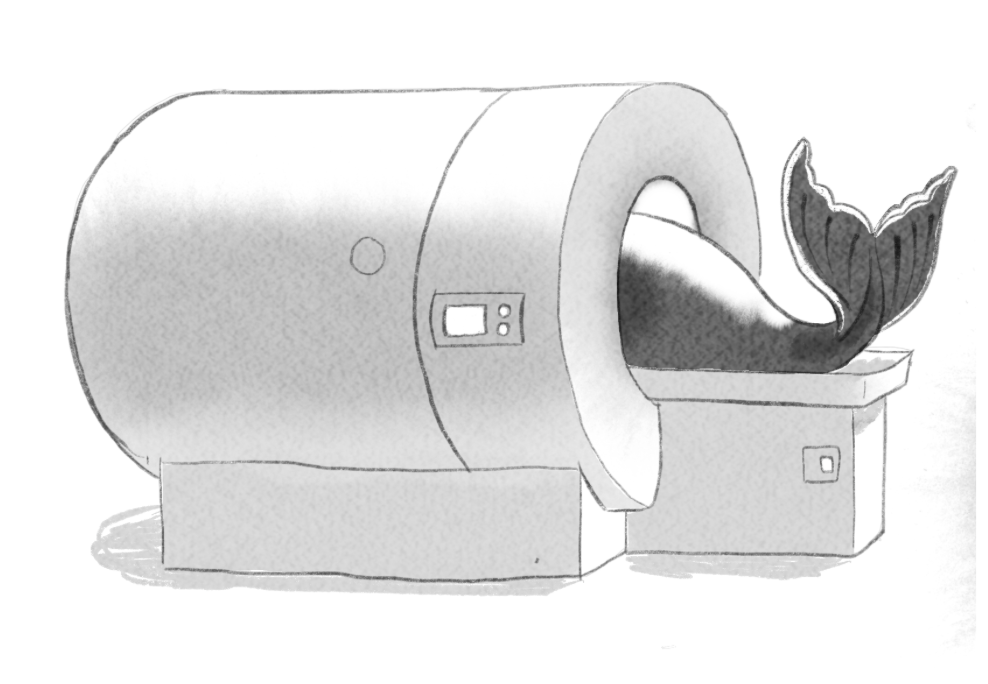
\includegraphics[width=1.5cm]{complexwhale}
		\vspace{2em}
	\end{minipage}
	
}
\makeatother

%%%%%

\title[Brainwise Wordsearch]{Lexical Methodological Exploration of Neuroimaging Studies}
\subtitle[]{PoCS2 Project Proposal}

\date{}

\author[Tony Barrows]{Tony Barrows}

%\institute[UVM]{ 
\includegraphics[width=4cm]{larner}}

%\institute{\inst{1} University of Vermont \and \inst{2} University of Michigan}

\begin{document}
	
	\begin{frame}
		\maketitle
		
		\centering
%		\includegraphics[width=2cm]{../../../pres-images/20150925-ABCD}
		
\includegraphics[width=3cm]{larner}
		
\includegraphics[width=3cm]{nerve}
		
\includegraphics[width=2cm]{complexsystems}
		
\includegraphics[width=2cm]{complexbrain}
%		
\includegraphics[width=2cm]{../../../pres-images/complexsystems}
%		\includegraphics[width=3cm]{../../../pres-images/vacc_green}
	\end{frame}
	
	%% Outline
%\begin{frame}{Outline}
%	\tableofcontents
%\end{frame}

\begin{frame}{Motivation}

	Look for neurobiological mechanisms behind individual differences in behavior
	
	\begin{itemize}
		\item Chart normal and abnormal brain and cognitive development
		\item Identify biomarkers for abnormal behavior
		\item Afford opportunities for individualized medicine
	\end{itemize}

	\begin{block}{}
		Use neuroimaging to help us understand brain-behavior relationships
	\end{block}
\end{frame}

\begin{frame}{Problem}
	\begin{columns}
		\column{0.2\textwidth}
		\includegraphics[width=\columnwidth]{papers/Marek22}
		\column{0.8\textwidth}
		\textbf{Reproducible brain-wide association studies require thousands of individuals \cite{MarekEtAl2022}}
		
		Reasons:
		\begin{itemize}
			\item Fishing for statistical significance (``p-hacking'') \cite{Nuzzo}
			\item Overfitting \cite{Hawkins2004}
			\item Confirmation and publication biases \cite{Bishop2020}
			\item Variability in methods \cite{Botvinik-NezerEtAl2020}
		\end{itemize}
	\end{columns}
\end{frame}

%TODO Add basic neuroimaging study overview

\begin{frame}{Overview}
		(Very) High-level overview of Functional Magnetic Resonance Imaging (fMRI):
		
		\begin{itemize}
			\item Participants complete tasks in the scanner
			\item We measure changes in very small magnetic fields related to metabolic demand (blood flow after neuronal activity)
			\item Recording those changes over time creates a time-series for each tiny volume (voxel)
			\item Use GLMs to relate the task to the brain time-series
			\item Fit additional models to look for group-level differences
			\item Draw pictures using these models
		\end{itemize}
		
		\begin{figure}
				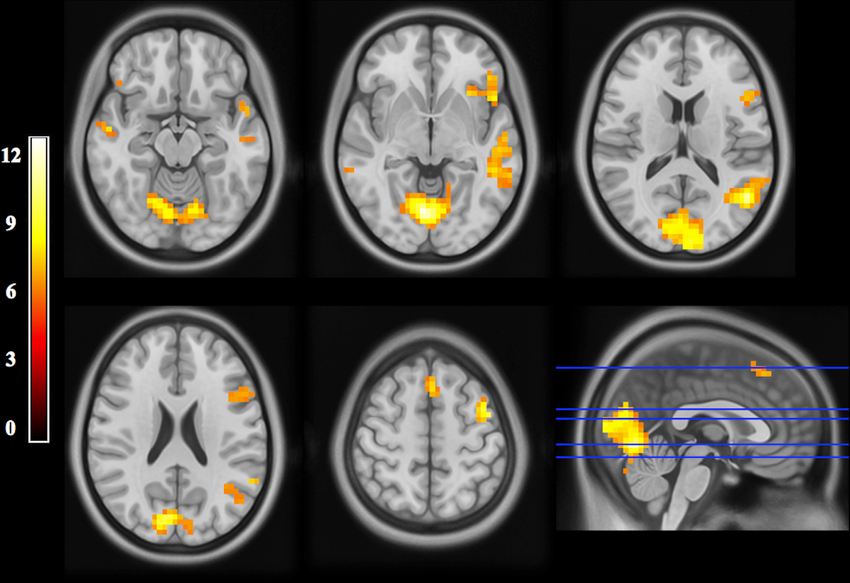
\includegraphics[width=0.3\textwidth]{fmri_ex}
				\caption{fMRI group-level activation map from \cite{VassalEtAl2016}.}
		\end{figure}


\end{frame}



% TODO describe goal
% TODO Introduce datasets


\begin{frame}[allowframebreaks]{References}

		\tiny
		\bibliography{zotero}

\end{frame}


	
	
\end{document}

